\documentclass[a4paper]{article}
\usepackage{cmap}
\usepackage{mathtext}
\usepackage{amssymb}
\usepackage{amsmath}
\usepackage{wrapfig}
\usepackage[russian]{babel}
\usepackage{indentfirst}
\usepackage[pdftex]{graphicx}
\usepackage{multirow}
\usepackage{mathrsfs}
\usepackage{biblatex}
\usepackage{siunitx}
\usepackage[left=2cm,right=2cm,top=2cm,bottom=2cm]{geometry}
\usepackage{fancyhdr}
\bibliography{bib}
\pagestyle{fancy}
\newcommand{\const}{\mathrm{const}}
\newcommand{\rref}[1]{(\ref{#1})}
\newcommand{\isotope}[2]{$ ^{#2}\mathrm{#1} $}
\newenvironment{comment}{}{}
\newcommand{\picref}[1]{рис. \ref{#1}}
\newcommand{\mbf}{\mathbf}
\newcommand{\gmm}{$\gamma $}
\newcommand{\Equip}[3]{
	
	\item{\bf #1:} $\Delta = \pm #2\; #3$}
\newcommand{\equip}[1]{
	
	\item{\bf #1}}
\newcommand{\labname}{Компьютерная сцинтилляционная \gmm-спектрометрия} 	% название пиши здесь
\newcommand{\labnum}{5.5.5}		% номер вводи здесь
\fancyfoot{}
\fancyhead[RE, RO]{\thepage}
\fancyhead[LE, LO]{Лабораторная работа \labnum \space \labname}
\title{Лабораторная работа \labnum \space \labname}
\author{Иван Сладков}
\begin{document}
\maketitle
\thispagestyle{empty}
\section{Аннотация}
В данной работе проводится исследование спектров \gmm-лучей от различных образцов при помощи сцинтилляционных \gmm-спектрометров на основе неорганического кристалла NaI(Tl) и органической сцинтиллирующей пластмассы. 

\section{Теоретические сведения}

\paragraph{Взаимодействие с веществом}

При прохождении \gmm-квантов через материальную среду образуются электроны, возникающие за счет фотоэффекта, комптоновского рассеяния и рождения электрон-позитронных пар. Образующиеся при этих процессах электроны испытывают большое количество неупругих соударений с молекулами и атомами среды. Неупругие соударения могут сопровождаться как ионизацией, так и возбуждением молекул или атомов среды. При переходах возбужденных молекул или атомов в основное состояние, при рекомбинации электрических зарядов и т.п. в веществе возникают кванты света различных длин волн, присущих данному веществу. 

Вообще говоря, возникающее излучение должно сильно поглощаться в сцинтилляторе, так как его энергия в точности равна энергии возбуждения атомов среды. Чтобы избежать этого явления, в кристаллы сцинтиллятора вводят небольшие добавки других атомов. При этом спектр поглощения сдвигается относительно спектра испускания в сторону меньших длин волн, и увеличивается вероятность выхода из вещества хотя бы некоторой части квантов света, отвечающих длинноволновому краю спектра испускания. В этом случае прохождение ионизирующей частицы через вещество будет сопровождаться световой вспышкой, которая и может быть использована для регистрации частицы. 

\paragraph{Энергетическое разрешение спектрометра}

Даже при поглощении частиц с одинаковой энергией амплитуда импульса на выходе фотоприёмника сцинтилляционного детектора меняется от события к событию. Это связано со статистическим характером процессов сбора фотонов на фотоприёмнике и последующего усиления, с различной вероятностью доставки фотона к фотоприёмнику из разных точек сцинтиллятора и с разбросом высвечиваемого числа фотонов. Поэтому линия на спектре размывается. Её часто описывают гауссианом. В данной работе используется этот метод обработки данных. 

Энергетическим разрешением спектрометра называется величина
\begin{equation}
	R_i = \dfrac{\Delta E_i}{E_i} \propto \dfrac{1}{\sqrt{E_i}}.
\end{equation}
Здесь $ \Delta E_i $ -- ширина пика полного поглощения, измеренная на половине высоты. Энергетическое разрешение, очевидно, зависит от энергии, поэтому чаще всего его указывают для энергии \gmm-линии \isotope{Cs}{137}.

\subsection{Расчётные формулы}

Для эффекта Комптона значение энергии \gmm-кванта после взаимодействия определяется по формуле
\begin{equation*}\label{ы}
	E' = \frac{E}{1+\frac{E}{m c^2}\left( 1- \cos \theta\right) }
\end{equation*}

Форма импульсов на выходе ФЭУ определяется выражением
\begin{equation}\label{eq:2}
	U(t)\propto e^{-\frac{1}{R C}}\left( 1 - e^{-\frac{t}{\tau_0}}\right).
\end{equation}

\section{Оборудование и инструментальные погрешности}

Схема экспериментальной установки отображена на рис. \ref{fig:screenshot1}.
\begin{figure}
	\centering
	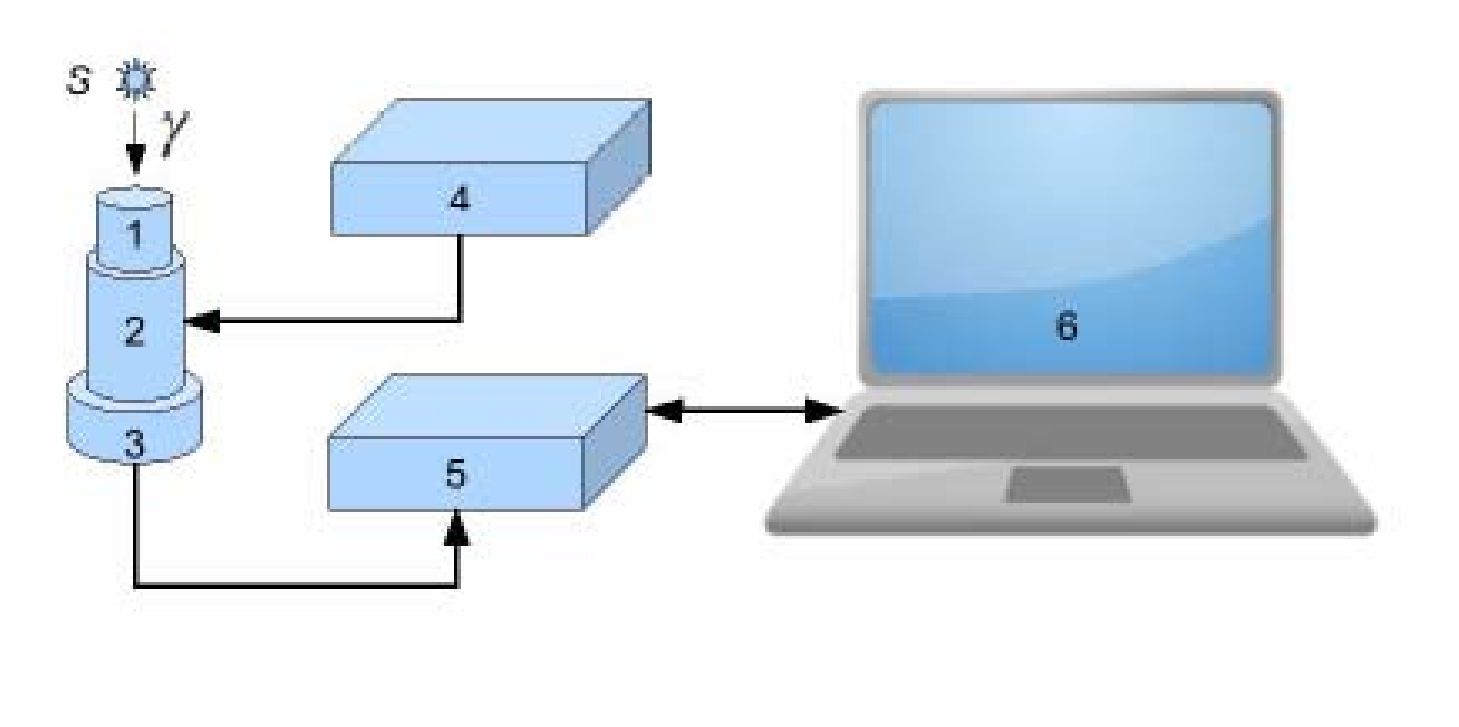
\includegraphics[width=0.7\linewidth]{Screenshot_1}
	\caption{Принципиальная схема экспериментальной установки}
	\label{fig:screenshot1}
\end{figure}


В работе используются:
\begin{itemize}
	\equip{Сцинтиллятор}
	\equip{Фотоэлектронный умножитель (ФЭУ)}
	\equip{Предусилитель импульсов}
	\equip{Высоковольтный блок питания ФЭУ}
	\equip{Блок АЦП}
	\equip{Компьютер для сбора данных}
\end{itemize}

\section{Результаты измерений и обработка данных}

После проверки работоспособности приборов и калибровки проведём измерение фона. Соответствующий спектр отображён на рис. \ref{fig:фон}.

Также найдём и проанализируем пики полного поглощения для веществ \isotope{Na}{22}, \isotope{Co}{60}, \isotope{Cs}{137}, \isotope{Eu}{152} и \isotope{Am}{241}. Результаты анализа и апроксимации пиков отображены на рис. \ref{fig:Na}-\ref{fig:Am} соответственно.
\begin{figure}
	\centering
	\includegraphics[width=0.7\linewidth]{"1"}
	\caption{Пики полного поглощения для \isotope{Na}{22}}
	\label{fig:Na}
\end{figure}
\begin{figure}
	\centering
	\includegraphics[width=0.7\linewidth]{"2"}
	\caption{Пики полного поглощения для \isotope{Co}{60}}
	\label{fig:Co}
\end{figure}
\begin{figure}
	\centering
	\includegraphics[width=0.7\linewidth]{"3"}
	\caption{Пики полного поглощения для \isotope{Cs}{137}}
	\label{fig:Cs}
\end{figure}
\begin{figure}
	\centering
	\includegraphics[width=0.7\linewidth]{"4"}
	\caption{Пики полного поглощения для \isotope{Eu}{152}}
	\label{fig:Eu}
\end{figure}
\begin{figure}
	\centering
	\includegraphics[width=0.7\linewidth]{"5"}
	\caption{Пики полного поглощения для \isotope{Am}{241}}
	\label{fig:Am}
\end{figure}

В каждом спектре определим номера каналов, отвечающие центрам пиков полного поглощения излучения от радиоактивных источников \isotope{Na}{22} и \isotope{Cs}{137}. Этим каналам присваивают соответствующие табличные значения энергий и проводят линейную аппроксимацию зависимости энергии от номера канала для данного $\gamma$-спектрометра при данной геометрии измерения и настройках $\gamma$-спектрометра. Построим калибровочный график зависимости номера канала от энергии $\gamma$-кванта на рис. \ref{fig:calibre}.
\begin{figure}
	\centering
	\begin{minipage}{0.49\linewidth}
		\centering
		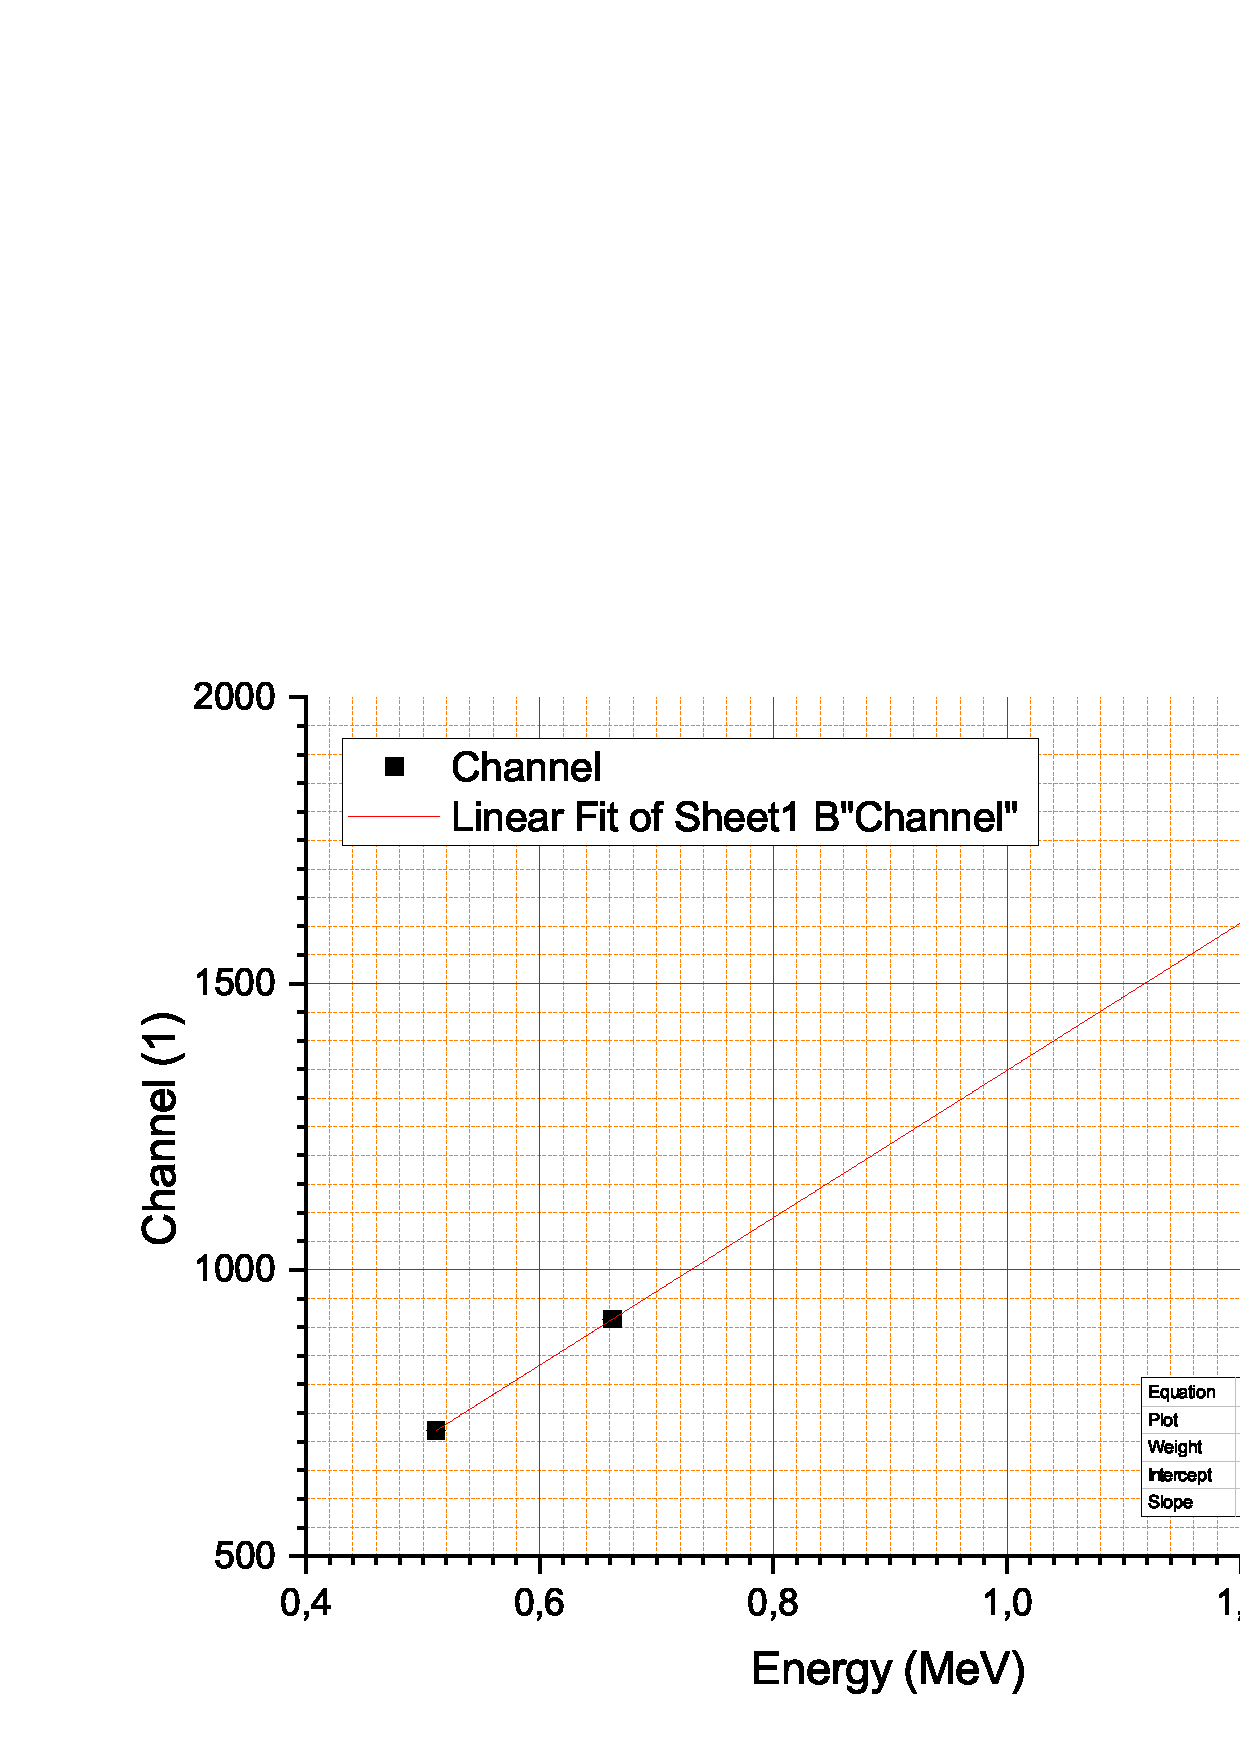
\includegraphics[width=1\linewidth]{calibre}
		\caption{Калибровочный график $N_i = a + b E_i $}
		\label{fig:calibre}
	\end{minipage}
	\hfill
	\begin{minipage}{0.49\linewidth}
				\centering
		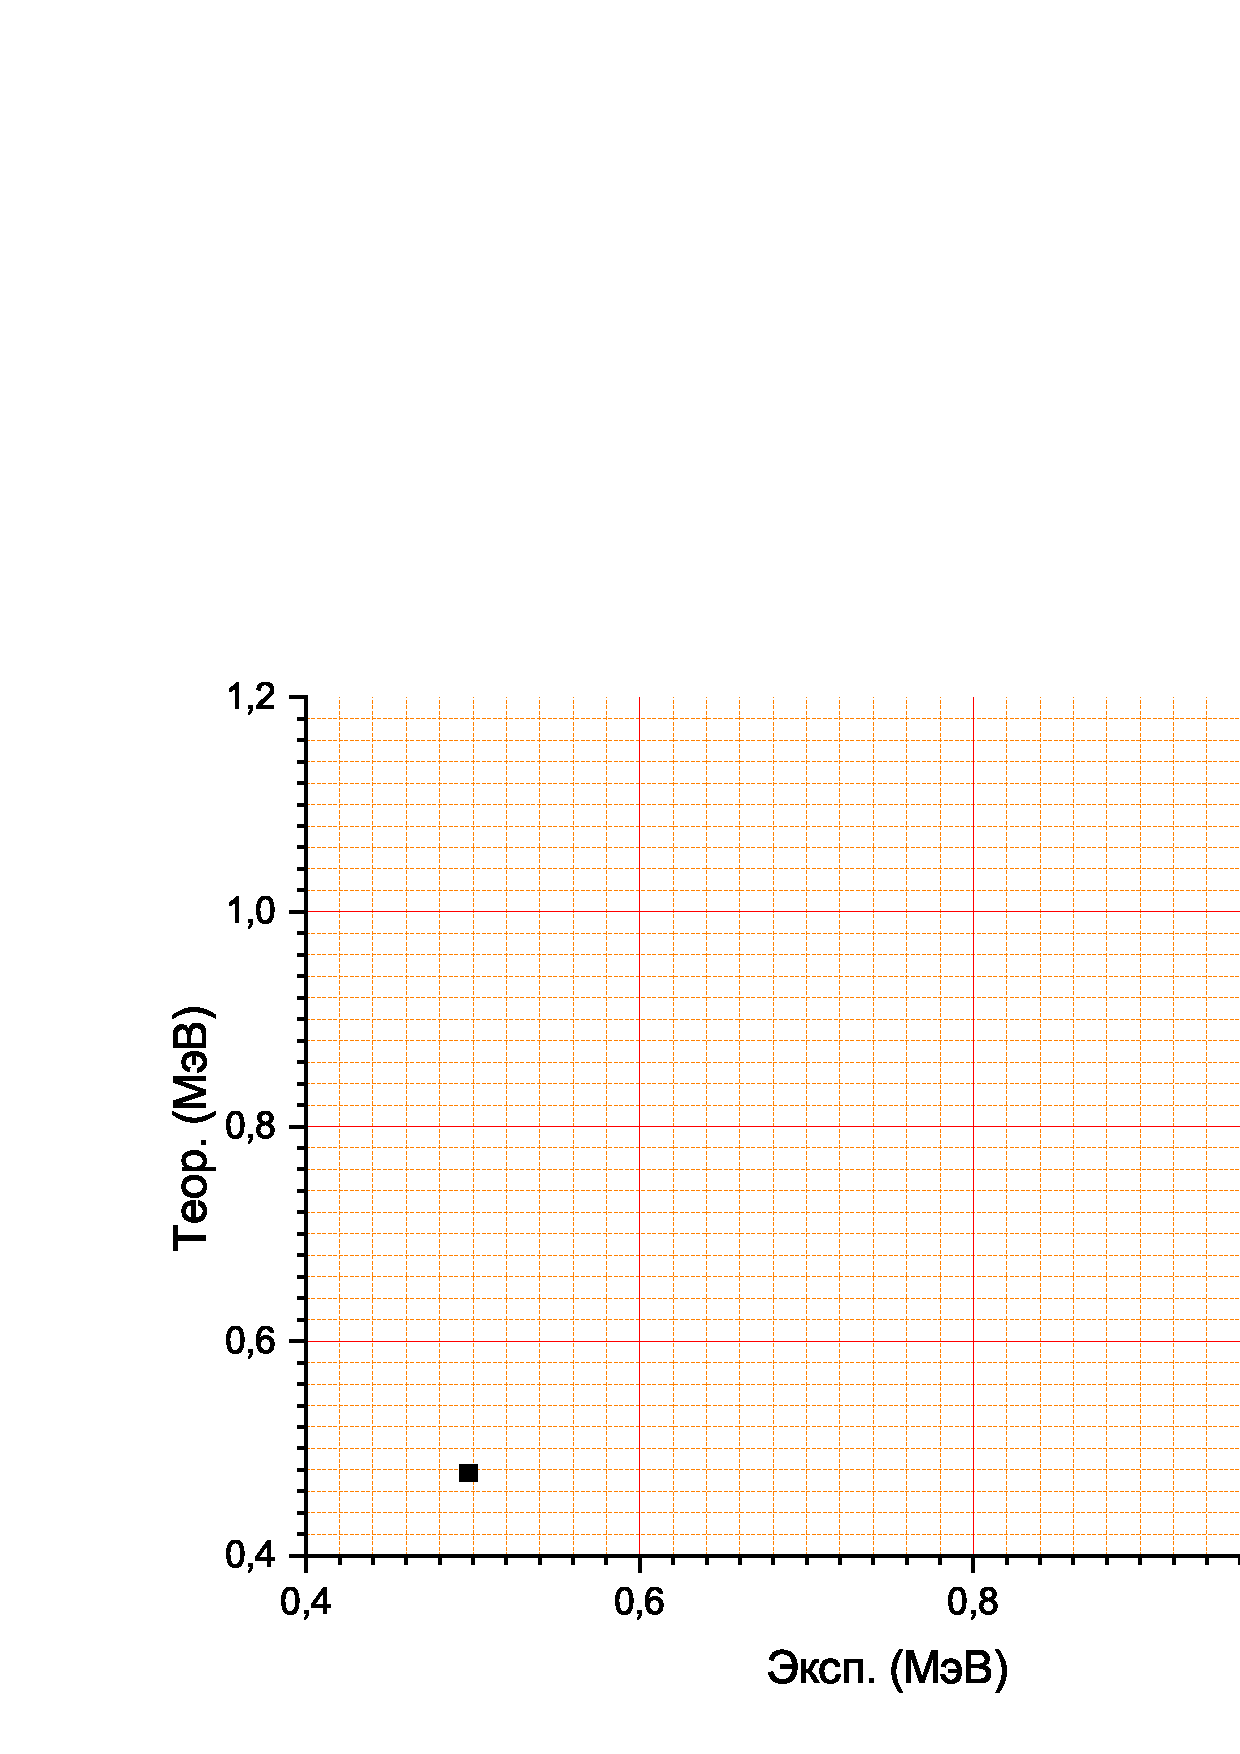
\includegraphics[width=1\linewidth]{Сравнение}
		\caption{Сравнение теоретических и практических значений максимальной энергии при эффекте Комптона}
		\label{fig:comp}
	\end{minipage}
\end{figure}
Из него можно получить формулу для энергии: $ E_i = N_i/1286 - 0.047 $ МэВ. Используя калибровочный график, определим для всех остальных источников значения энергии пиков полного поглощения $ E_i $, их ширины на половине высоты $\Delta E_i$ и энергетическое разрешение $ R_i $ . Результаты сохраним в таблице \ref{tab:1}.
\begin{table}[]
	\centering
	\begin{tabular}{|l|l|l|l|l|l|}
		\hline
		Источник & $N_i$ & $\Delta N_i$ & $E_i,$ МэВ & $\Delta E_i,$ МэВ & $R_i$ \\ \hline
		\multirow{2}{*}{\isotope{Na}{22}}  & 719$\pm$1  & 50.3$\pm$0.5 & 0.511$\pm$0.001 & 0.038$\pm$0.001  & 0.070$\pm$0.001 \\ \cline{2-6} 
		& 1695$\pm$2 & 68$\pm$4 & 1.274$\pm$0.003 & 0.051$\pm$0.003  & 0.040$\pm$0.004 \\ \hline
		\multirow{2}{*}{\isotope{Co}{60}}  & 1567$\pm$1 & 75$\pm$1 & 1.168$\pm$0.001 & 0.058$\pm$0.001 & 0.049$\pm$0.002 \\ \cline{2-6} 
		& 1771$\pm$1 & 80$\pm$2 & 1.327$\pm$0.001 & 0.062$\pm$0.002 & 0.047$\pm$0.003 \\ \hline
		\isotope{Cs}{137}                  & 914$\pm$1  & 57$\pm$1 & 0.662$\pm$0.001 & 0.044$\pm$0.001 & 0.066$\pm$0.001 \\ \hline
		\multirow{2}{*}{\isotope{Eu}{152}} & 114.8$\pm$0.1  & 15$\pm$1 & 0.039$\pm$0.001 & 0.011$\pm$0.001 & 0.280$\pm$0.003 \\ \cline{2-6} 
		& 227$\pm$1  & 15$\pm$0.5 & 0.126$\pm$0.001 & 0.011$\pm$0.002 & 0.081$\pm$0.001 \\ \hline
		\multirow{2}{*}{\isotope{Am}{241}} & 145.5$\pm$0.5  & 11$\pm$1 & 0.0630$\pm$0.0005 & 0.008$\pm$0.001 & 0.128$\pm$0.002 \\ \cline{2-6} 
		& 99.3$\pm$0.5   & 14.1$\pm$0.5 & 0.027$\pm$0.001 & 0.0103$\pm$0.0005 & 0.370$\pm$0.002  \\ \hline
	\end{tabular}
	\caption{Сводная таблица пиков}
	\label{tab:1}
\end{table}

По результатам измерения энергии края комптоновского поглощения (табл. \ref{tab:2}) построим график \ref{fig:comp}, по одной оси которого отложим экспериментальные значения, а по другой -- расчетные значения этой энергии. 
\begin{table}[h]
	\centering
	\begin{tabular}{|l|l|l|}
		\hline
		\multirow{2}{*}{} & \multicolumn{2}{l|}{$E_{\mathrm{Комп. max}}$, МэВ} \\ \cline{2-3} 
		& Эксп.                   & Теор.                   \\ \hline
		\isotope{Na}{22}  & 1.041                   & 1.062                   \\ \hline
		\isotope{Co}{60}  & 1.002                   & 0.963                   \\ \hline
		\isotope{Cs}{137} & 0.497                   & 0.477                   \\ \hline
	\end{tabular}
	\caption{Результаты измерения энергии края комптоновского поглощения}
	\label{tab:2}
\end{table}

Для проверки зависимости (1), построим по полученным данным график \ref{fig:10}. Значение минимальной энергии для \isotope{Am}{241} исключим из рассмотрения из-за большой погрешности.
\begin{figure}
	\centering
	\begin{minipage}{0.49\linewidth}
		\centering
		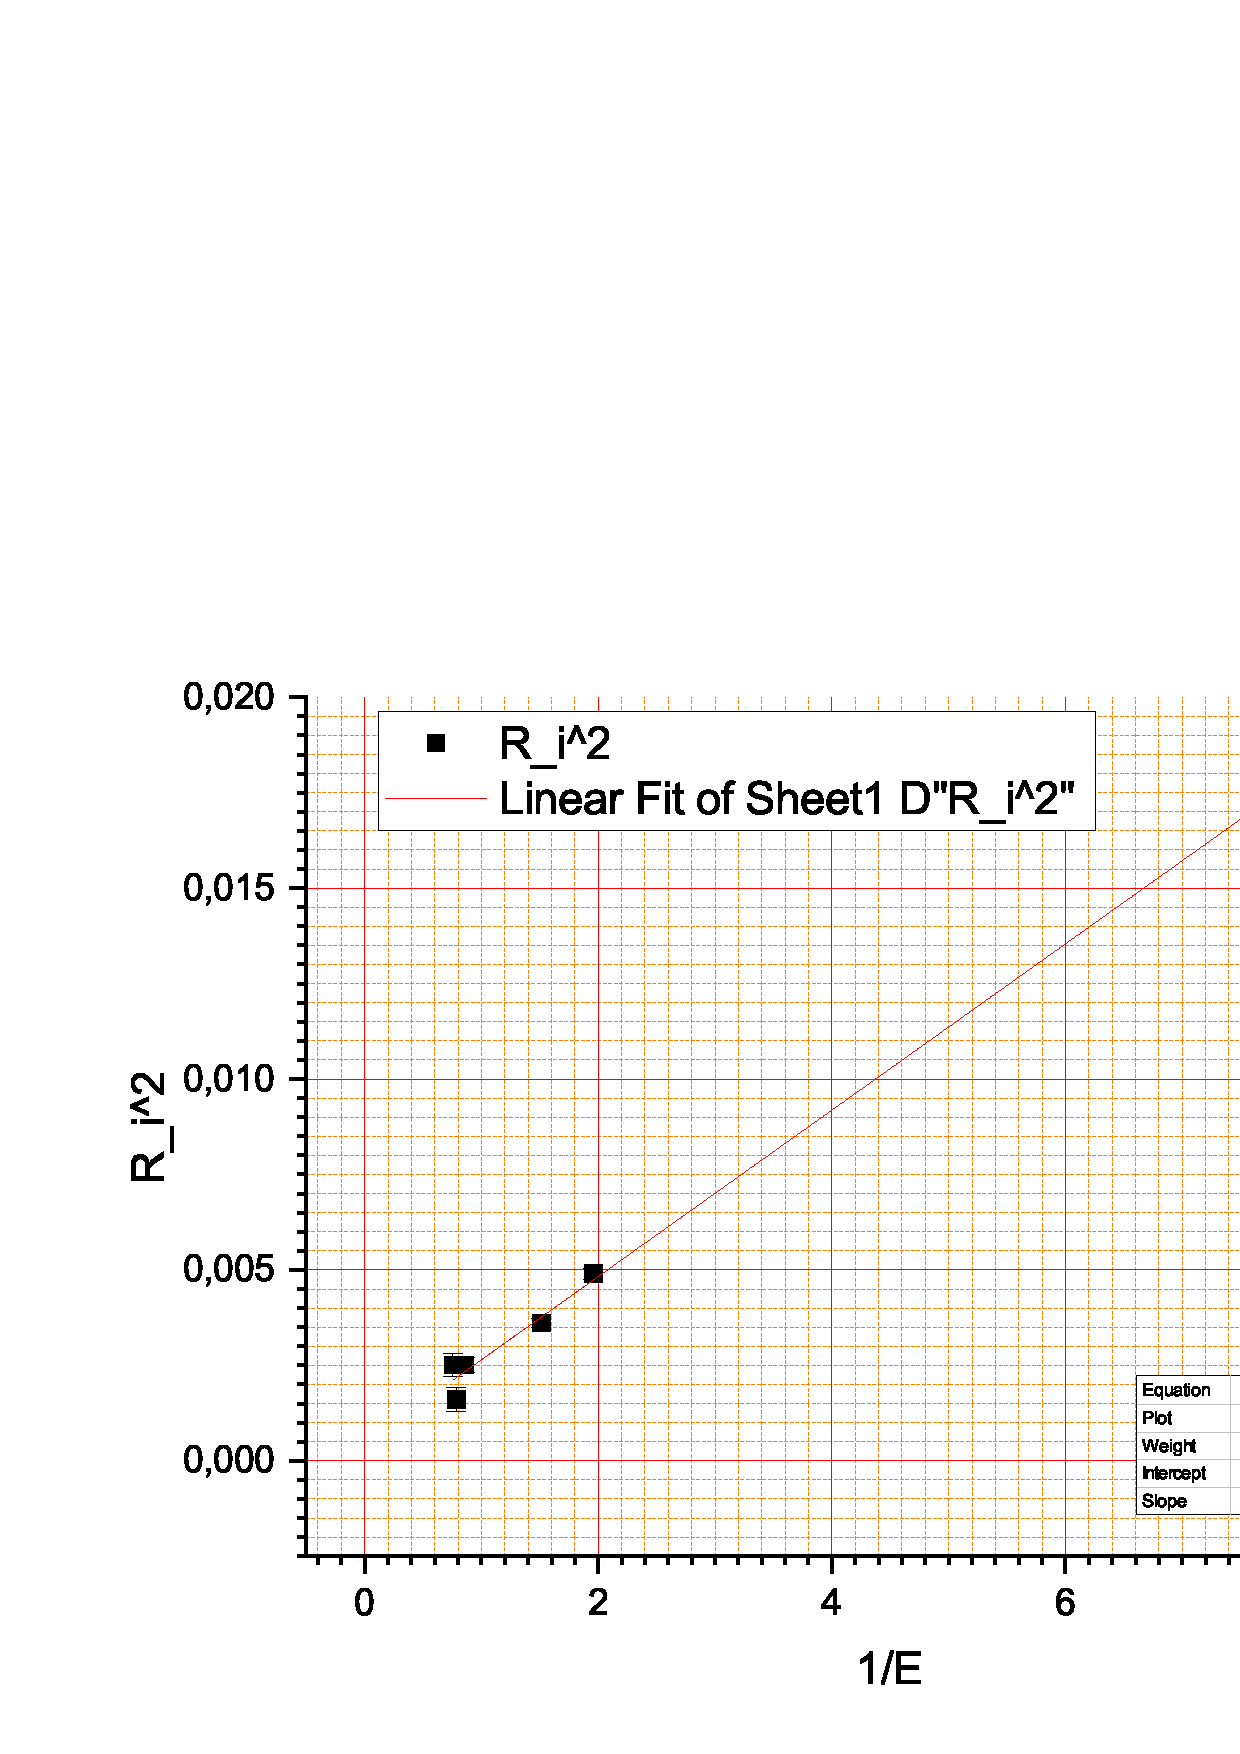
\includegraphics[width=0.9\linewidth]{Graph15}
		\caption{График зависимости $R_i = f (1/E_i)$}
		\label{fig:10}
	\end{minipage}
	\begin{minipage}{0.49\linewidth}
		\centering
		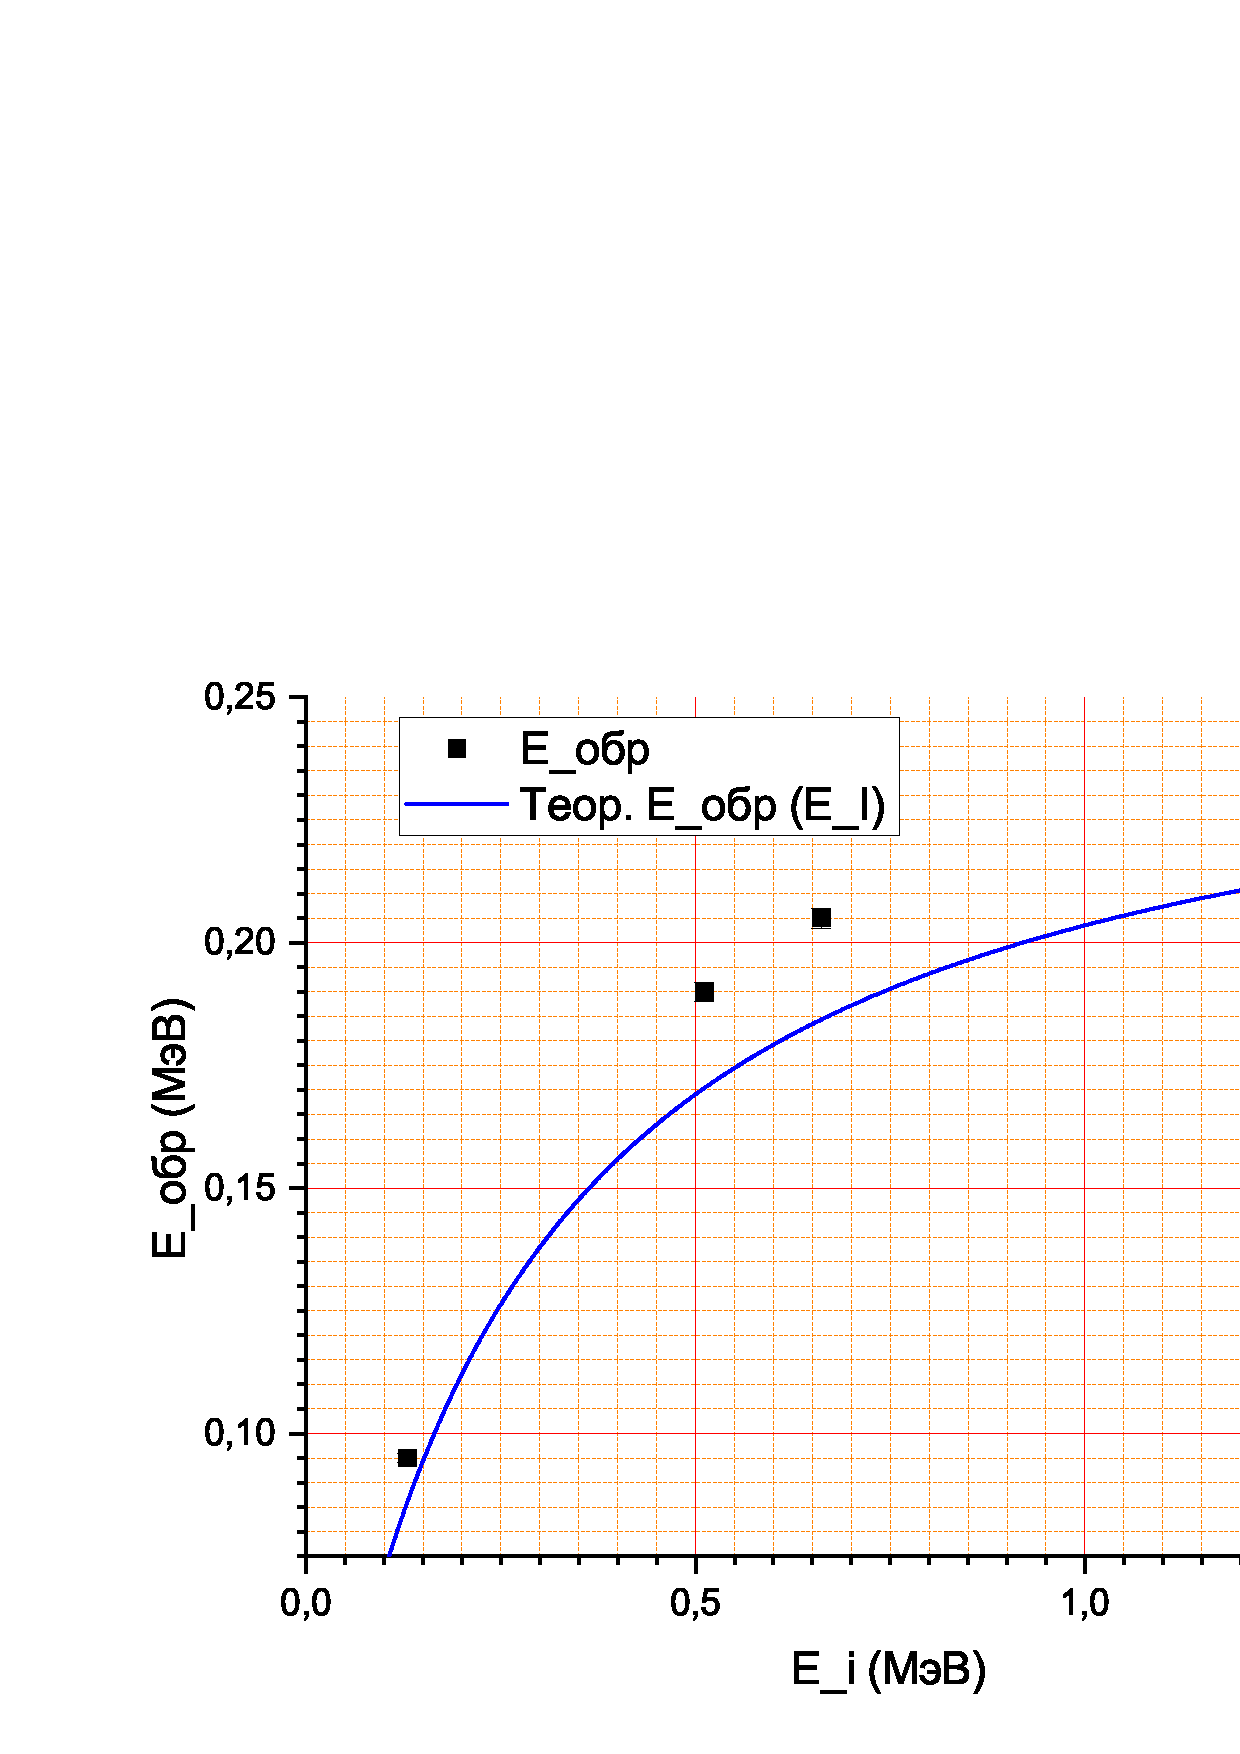
\includegraphics[width=0.9\linewidth]{Graph17}
		\caption{Теоретическая и экспериментальная зависимости $E_{обр} = f (E_i)$}
		\label{fig:last}
	\end{minipage}
\end{figure}

Далее, построим график зависимости энергии пика обратного рассеяния от энергии на рис. \ref{fig:last}.

По данным осциллографа, отображённым на рис. \ref{fig:screenshot2}, где виден импульс от высокоэнергетической частицы, из соотношения \eqref{eq:2} оценим величины $\tau_0$ и $ R C $ по переднему и заднему фронтам импульса соответственно
\[
	\tau_0\approx 0.8\; мс,
\]
\[
	R C \approx 2\; мс.
\]
\begin{figure}
	\centering
	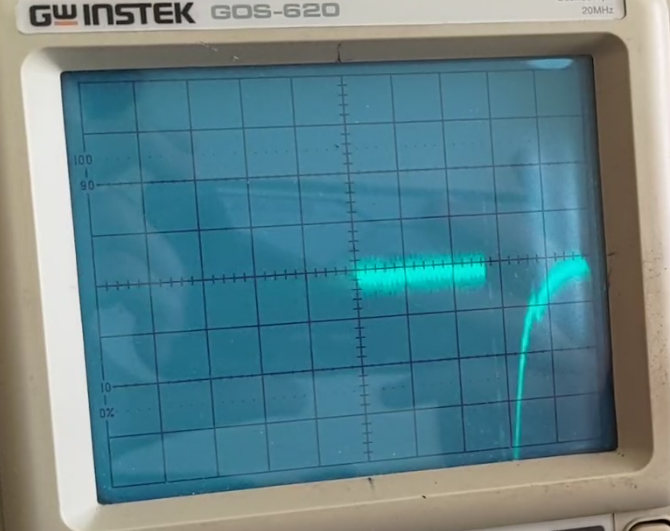
\includegraphics[width=0.7\linewidth]{Screenshot_2}
	\caption{Импульс от высокоэнергетической частицы на экране осциллографа}
	\label{fig:screenshot2}
\end{figure}

 
\subsection{Оценка погрешностей}
В данной работе крайне сложно проводить оценку погрешностей по причине характера исходных данных. В частности, не представляется возможным сделать оценку инструментальных погрешностей. Поэтому все оценки погрешностей проводились исключительно из статистических соображений, посчитаны из апроксимации пиков и являются существенно заниженными. Погрешности косвенных измерений рассчитаны по стандартной формуле.

\section{Вывод}
В ходе работы после калибровки прибора были сняты спектры образцов $^{22}$Na,  $^{60}$Cо,  $^{137}$Cs, $^{241}$Am, $^{152}$Eu. В спектрах были исследованы пики, соответствующие следующим взаимодействиям гамма-квантов с веществом:
\begin{itemize}
	\item фотоэффект (пики полного поглощения)
	\item эффект Комптона (характерное распределение энергий в спектре, оканчивающееся комптоновским краем)
	\item обратное рассеяние (пики обратного рассеяния)
	\item аннигиляция позитронов (пик 511 кэВ в спектре натрия, по которому проводилась калибровка)
\end{itemize}

Также была проверена линейная зависимость квадрата спектрального разрешения прибора от величины, обратной энергии полного поглощения.

Проведено сравнение спектров \isotope{Cs}{137} для двух разных сцинтилляторов: на красталлах NaI(Tl) и на органической сцинтиллирующей пластмассе. Также даны оценки характеристик экспериментальной установки -- времени высвечивания сцинтиллятора, а также постоянной времени анодной цепи ФЭУ.

\appendix
\section{Необработанные результаты опытов}

Спектры, полученные по результатам проведения опытов, представлены на рис. \ref{fig:first}-\ref{fig:фон}.

\begin{figure}
	\begin{center}
		\begin{minipage}{0.49\linewidth}
			\includegraphics[width=1\linewidth]{na.eps}
			\caption{Спектр $^{22}$Na} %% подпись к рисунку\label{ris:experimoriginal} %% метка рисунка для ссылки на него
			\label{fig:first}
		\end{minipage}
		\hfill 
		\begin{minipage}{0.49\linewidth}
			\includegraphics[width=1\linewidth]{co.eps}
			\caption{Спектр $^{60}$Co}
			\label{ris:experimcoded}
		\end{minipage}
		\begin{minipage}{0.49\linewidth}
			\includegraphics[width=1\linewidth]{eu.eps}
			\caption{Спектр $^{152}$Eu} %% подпись к рисунку\label{ris:experimoriginal} %% метка рисунка для ссылки на него
		\end{minipage}
		\hfill 
		\begin{minipage}{0.49\linewidth}
			\includegraphics[width=1\linewidth]{am.eps}
			\caption{Спектр $^{241}$Am}
			\label{ris:xperimcoded}
		\end{minipage}
		\begin{minipage}{0.49\linewidth}
			\includegraphics[width=1\linewidth]{cs.eps}
			\caption{Спектр $^{137}$Cs} %% подпись к рисунку\label{ris:experimoriginal} %% метка рисунка для ссылки на него
		\end{minipage}
		\hfill 
		\begin{minipage}{0.49\linewidth}
			\includegraphics[width=1\linewidth]{cs_diff.eps}
			\caption{Спектр $^{137}$Cs с другой установки}
			\label{ris:xperimcode}
		\end{minipage}
	\end{center}
\end{figure}
\begin{figure}
	\centering
	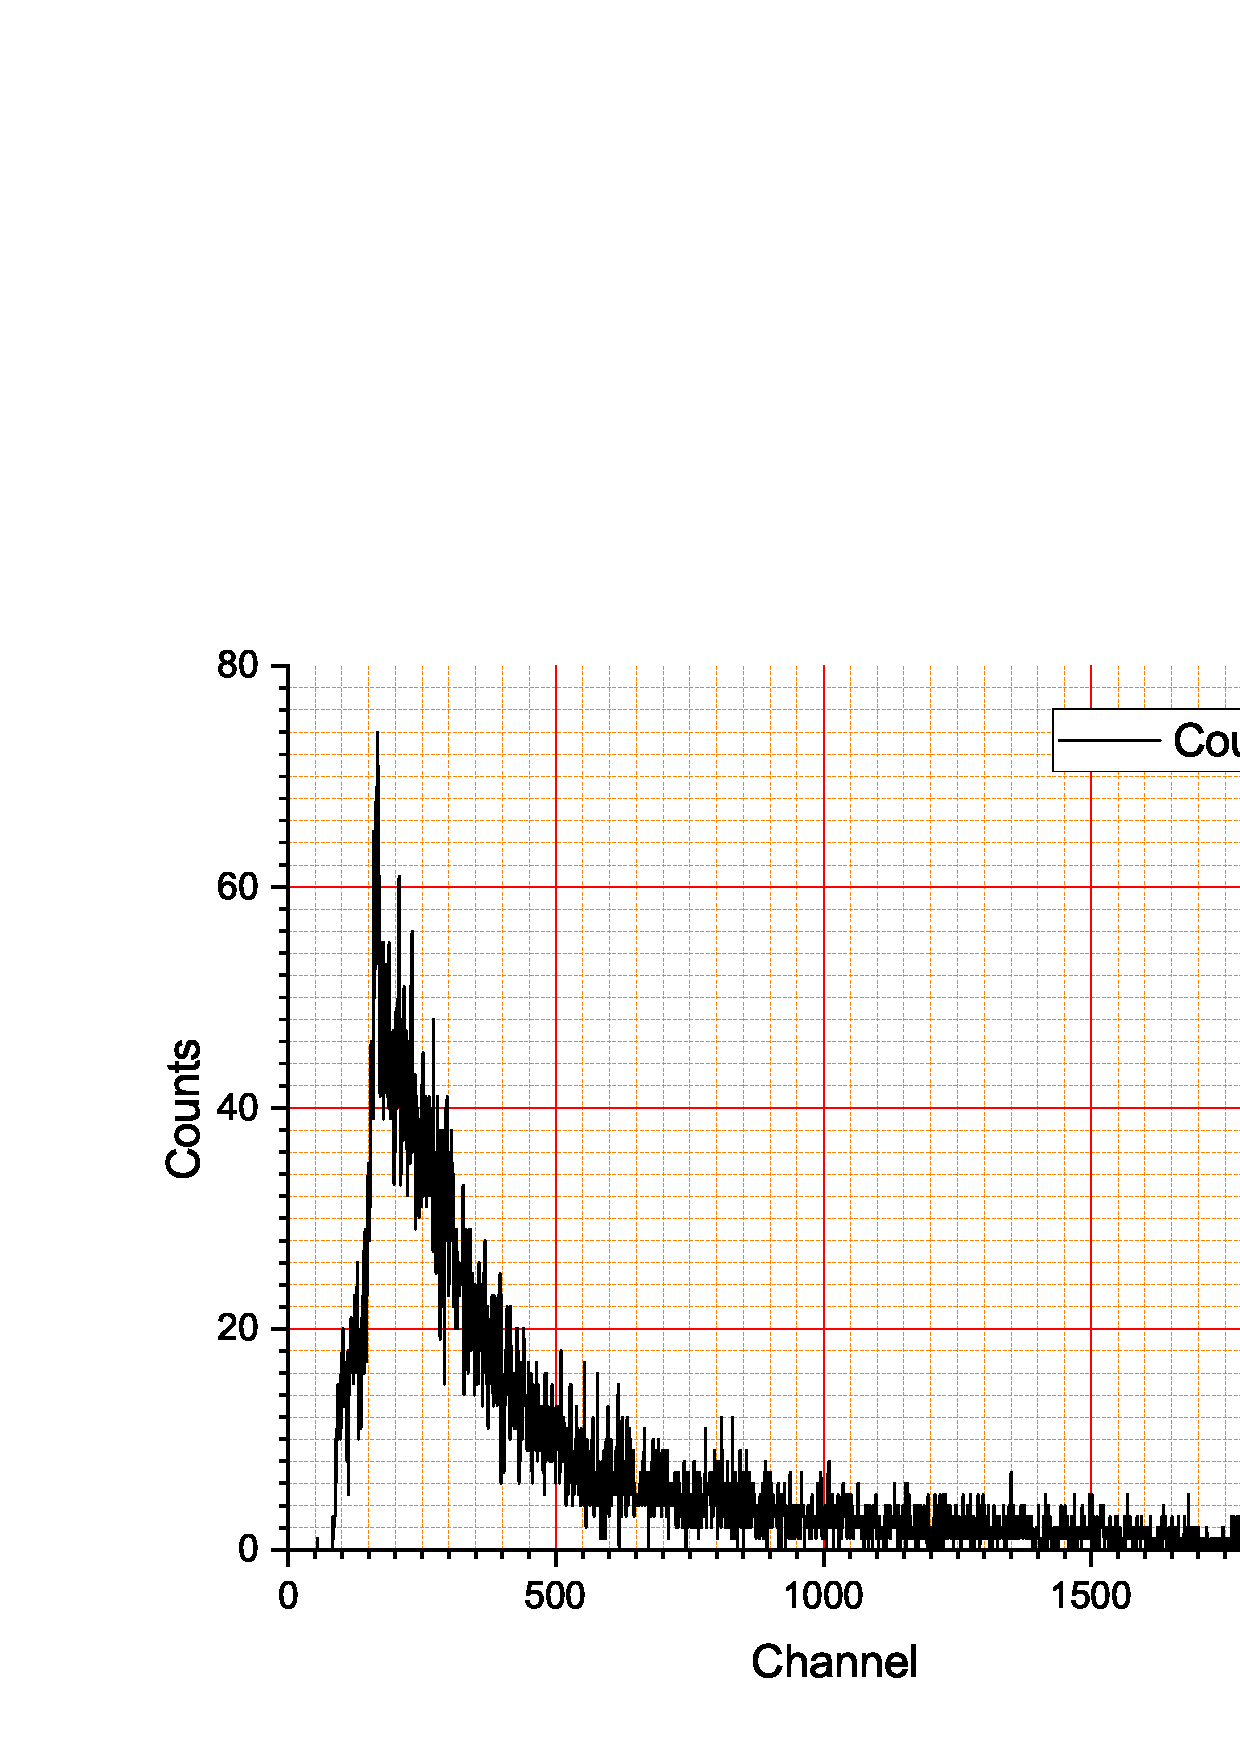
\includegraphics[width=0.49\linewidth]{фон}
	\caption{Спектр, соответствующий фону}
	\label{fig:фон}
\end{figure}

\newpage
\begin{thebibliography}{9}
	\bibitem{Siv} Сивухин Д. В. \emph{Общий курс физики. Том 4 Оптика}, 2004
	\bibitem{kir} Кириченко Н. А. \emph{Принципы оптики}, 2014
	\bibitem{max} \emph{Лабораторный практикум по общей физике. В 3 томах. Том 2. Оптика: учебное пособие} под ред. А. В. Максимычева
\end{thebibliography}
\end{document}